\subsection{Software}
We develop a software package with a user interface that implements the above LP problem and allows configuration of clinicians at [ref \ref{???}], to be used by the ID division at St. Michael's Hospital. The software was used to generate the results in the following sections, using real data as well as simulated data as input.

\subsection{Infectious Diseases Division}
We use clinician time-off requests and minimum/maximum requirements from 2015-2018 as input data for the LP problem. Tables \ref{tbl:2017-schedule-comparison}, \ref{tbl:2018-schedule-comparison}, \ref{??}, \ref{??} present the optimal schedule generated using the software as well as the manually created schedule, color-coded to distinguish between the different clinicians assigned.

% Table generated by Excel2LaTeX from sheet '2017'
\begin{table}[h]
	\tiny
	\centering
    \begin{tabular}{c||ccc||ccc}
    	\multicolumn{1}{c||}{\multirow{2}[1]{*}{Week \#}} & \multicolumn{3}{c||}{LP Solution}                                                                                                                                                              & \multicolumn{3}{c}{Historical Data}                                                                                                                                                            \\
    	                                                  &                             HIV                             &                                 ID                                 &                              Weekend                               &                             HIV                             &                                 ID                                 &                              Weekend                               \\ \midrule\midrule
    	                        1                         &            \cellcolor[rgb]{ .608,  .761,  .902}B            &                  \cellcolor[rgb]{ 1,  .851,  .4}C                  &               \cellcolor[rgb]{ .608,  .761,  .902}B                &            \cellcolor[rgb]{ .663,  .816,  .557}A            &               \cellcolor[rgb]{ .788,  .788,  .788}D                &    \cellcolor[rgb]{ .6,  .2,  1}\textcolor[rgb]{ 1,  1,  1}{J}     \\
    	                        2                         &            \cellcolor[rgb]{ .608,  .761,  .902}B            &                  \cellcolor[rgb]{ 1,  .851,  .4}C                  &                \cellcolor[rgb]{ .957,  .69,  .518}E                &            \cellcolor[rgb]{ .663,  .816,  .557}A            &               \cellcolor[rgb]{ .788,  .788,  .788}D                &               \cellcolor[rgb]{ .557,  .663,  .859}F                \\
    	                        3                         &            \cellcolor[rgb]{ .663,  .816,  .557}A            &               \cellcolor[rgb]{ .557,  .663,  .859}F                &               \cellcolor[rgb]{ .557,  .663,  .859}F                &            \cellcolor[rgb]{ .608,  .761,  .902}B            &                \cellcolor[rgb]{ .518,  .592,  .69}G                &               \cellcolor[rgb]{ .663,  .816,  .557}A                \\
    	                        4                         &            \cellcolor[rgb]{ .663,  .816,  .557}A            &               \cellcolor[rgb]{ .557,  .663,  .859}F                &               \cellcolor[rgb]{ .663,  .816,  .557}A                &            \cellcolor[rgb]{ .608,  .761,  .902}B            &                \cellcolor[rgb]{ .518,  .592,  .69}G                &                \cellcolor[rgb]{ .518,  .592,  .69}G                \\
    	                        5                         &            \cellcolor[rgb]{ .608,  .761,  .902}B            &                \cellcolor[rgb]{ .518,  .592,  .69}G                &               \cellcolor[rgb]{ .608,  .761,  .902}B                &            \cellcolor[rgb]{ .663,  .816,  .557}A            &    \cellcolor[rgb]{ .6,  .2,  1}\textcolor[rgb]{ 1,  1,  1}{J}     &                \cellcolor[rgb]{ .957,  .69,  .518}E                \\
    	                        6                         &            \cellcolor[rgb]{ .608,  .761,  .902}B            &                \cellcolor[rgb]{ .518,  .592,  .69}G                & \cellcolor[rgb]{ .251,  .251,  .251}\textcolor[rgb]{ 1,  1,  1}{I} &            \cellcolor[rgb]{ .663,  .816,  .557}A            &    \cellcolor[rgb]{ .6,  .2,  1}\textcolor[rgb]{ 1,  1,  1}{J}     & \cellcolor[rgb]{ .251,  .251,  .251}\textcolor[rgb]{ 1,  1,  1}{I} \\
    	                        7                         & \cellcolor[rgb]{ .6,  .2,  1}\textcolor[rgb]{ 1,  1,  1}{J} &               \cellcolor[rgb]{ .557,  .663,  .859}F                &    \cellcolor[rgb]{ .6,  .2,  1}\textcolor[rgb]{ 1,  1,  1}{J}     &            \cellcolor[rgb]{ .608,  .761,  .902}B            &               \cellcolor[rgb]{ .557,  .663,  .859}F                &                \cellcolor[rgb]{ .957,  .69,  .518}E                \\
    	                        8                         & \cellcolor[rgb]{ .6,  .2,  1}\textcolor[rgb]{ 1,  1,  1}{J} &               \cellcolor[rgb]{ .557,  .663,  .859}F                &                \cellcolor[rgb]{ .518,  .592,  .69}G                &            \cellcolor[rgb]{ .608,  .761,  .902}B            &               \cellcolor[rgb]{ .557,  .663,  .859}F                &                  \cellcolor[rgb]{ 1,  .851,  .4}C                  \\
    	                        9                         &            \cellcolor[rgb]{ .663,  .816,  .557}A            &                \cellcolor[rgb]{ .957,  .69,  .518}E                &               \cellcolor[rgb]{ .663,  .816,  .557}A                & \cellcolor[rgb]{ .6,  .2,  1}\textcolor[rgb]{ 1,  1,  1}{J} &                  \cellcolor[rgb]{ 1,  .851,  .4}C                  &    \cellcolor[rgb]{ .6,  .2,  1}\textcolor[rgb]{ 1,  1,  1}{J}     \\
    	                       10                         &            \cellcolor[rgb]{ .663,  .816,  .557}A            &                \cellcolor[rgb]{ .957,  .69,  .518}E                &                \cellcolor[rgb]{ .957,  .69,  .518}E                &            \cellcolor[rgb]{ .663,  .816,  .557}A            &                  \cellcolor[rgb]{ 1,  .851,  .4}C                  &               \cellcolor[rgb]{ .788,  .788,  .788}D                \\
    	                       11                         &            \cellcolor[rgb]{ .788,  .788,  .788}D            &               \cellcolor[rgb]{ .608,  .761,  .902}B                &               \cellcolor[rgb]{ .788,  .788,  .788}D                &            \cellcolor[rgb]{ .663,  .816,  .557}A            &               \cellcolor[rgb]{ .608,  .761,  .902}B                &               \cellcolor[rgb]{ .663,  .816,  .557}A                \\
    	                       12                         &            \cellcolor[rgb]{ .788,  .788,  .788}D            &               \cellcolor[rgb]{ .608,  .761,  .902}B                &                  \cellcolor[rgb]{ 1,  .851,  .4}C                  & \cellcolor[rgb]{ .6,  .2,  1}\textcolor[rgb]{ 1,  1,  1}{J} & \cellcolor[rgb]{ .251,  .251,  .251}\textcolor[rgb]{ 1,  1,  1}{I} & \cellcolor[rgb]{ .251,  .251,  .251}\textcolor[rgb]{ 1,  1,  1}{I} \\
    	                       13                         & \cellcolor[rgb]{ .6,  .2,  1}\textcolor[rgb]{ 1,  1,  1}{J} & \cellcolor[rgb]{ .251,  .251,  .251}\textcolor[rgb]{ 1,  1,  1}{I} & \cellcolor[rgb]{ .251,  .251,  .251}\textcolor[rgb]{ 1,  1,  1}{I} & \cellcolor[rgb]{ .6,  .2,  1}\textcolor[rgb]{ 1,  1,  1}{J} & \cellcolor[rgb]{ .251,  .251,  .251}\textcolor[rgb]{ 1,  1,  1}{I} &               \cellcolor[rgb]{ .557,  .663,  .859}F                \\
    	                       14                         & \cellcolor[rgb]{ .6,  .2,  1}\textcolor[rgb]{ 1,  1,  1}{J} & \cellcolor[rgb]{ .251,  .251,  .251}\textcolor[rgb]{ 1,  1,  1}{I} &    \cellcolor[rgb]{ .6,  .2,  1}\textcolor[rgb]{ 1,  1,  1}{J}     &            \cellcolor[rgb]{ .608,  .761,  .902}B            &               \cellcolor[rgb]{ .459,  .443,  .443}H                &                \cellcolor[rgb]{ .518,  .592,  .69}G                \\
    	                       15                         &            \cellcolor[rgb]{ .608,  .761,  .902}B            &                \cellcolor[rgb]{ .957,  .69,  .518}E                &                \cellcolor[rgb]{ .957,  .69,  .518}E                &            \cellcolor[rgb]{ .608,  .761,  .902}B            &               \cellcolor[rgb]{ .459,  .443,  .443}H                &               \cellcolor[rgb]{ .459,  .443,  .443}H                \\
    	                       16                         &            \cellcolor[rgb]{ .608,  .761,  .902}B            &                \cellcolor[rgb]{ .957,  .69,  .518}E                &               \cellcolor[rgb]{ .788,  .788,  .788}D                &              \cellcolor[rgb]{ 1,  .851,  .4}C               &                \cellcolor[rgb]{ .957,  .69,  .518}E                &    \cellcolor[rgb]{ .6,  .2,  1}\textcolor[rgb]{ 1,  1,  1}{J}     \\
    	                       17                         &            \cellcolor[rgb]{ .788,  .788,  .788}D            & \cellcolor[rgb]{ .251,  .251,  .251}\textcolor[rgb]{ 1,  1,  1}{I} & \cellcolor[rgb]{ .251,  .251,  .251}\textcolor[rgb]{ 1,  1,  1}{I} &              \cellcolor[rgb]{ 1,  .851,  .4}C               &                \cellcolor[rgb]{ .957,  .69,  .518}E                &                \cellcolor[rgb]{ .957,  .69,  .518}E                \\
    	                       18                         &            \cellcolor[rgb]{ .788,  .788,  .788}D            & \cellcolor[rgb]{ .251,  .251,  .251}\textcolor[rgb]{ 1,  1,  1}{I} &               \cellcolor[rgb]{ .557,  .663,  .859}F                &            \cellcolor[rgb]{ .663,  .816,  .557}A            &                \cellcolor[rgb]{ .518,  .592,  .69}G                &               \cellcolor[rgb]{ .557,  .663,  .859}F                \\
    	                       19                         &              \cellcolor[rgb]{ 1,  .851,  .4}C               &               \cellcolor[rgb]{ .459,  .443,  .443}H                &                  \cellcolor[rgb]{ 1,  .851,  .4}C                  &            \cellcolor[rgb]{ .663,  .816,  .557}A            &                \cellcolor[rgb]{ .518,  .592,  .69}G                &                \cellcolor[rgb]{ .518,  .592,  .69}G                \\
    	                       20                         &              \cellcolor[rgb]{ 1,  .851,  .4}C               &               \cellcolor[rgb]{ .459,  .443,  .443}H                &                \cellcolor[rgb]{ .518,  .592,  .69}G                & \cellcolor[rgb]{ .6,  .2,  1}\textcolor[rgb]{ 1,  1,  1}{J} &               \cellcolor[rgb]{ .557,  .663,  .859}F                &               \cellcolor[rgb]{ .663,  .816,  .557}A                \\
    	                       21                         &            \cellcolor[rgb]{ .663,  .816,  .557}A            &                \cellcolor[rgb]{ .957,  .69,  .518}E                &                \cellcolor[rgb]{ .957,  .69,  .518}E                &            \cellcolor[rgb]{ .788,  .788,  .788}D            &               \cellcolor[rgb]{ .557,  .663,  .859}F                &                  \cellcolor[rgb]{ 1,  .851,  .4}C                  \\
    	                       22                         &            \cellcolor[rgb]{ .663,  .816,  .557}A            &                \cellcolor[rgb]{ .957,  .69,  .518}E                & \cellcolor[rgb]{ .251,  .251,  .251}\textcolor[rgb]{ 1,  1,  1}{I} &            \cellcolor[rgb]{ .788,  .788,  .788}D            &                  \cellcolor[rgb]{ 1,  .851,  .4}C                  & \cellcolor[rgb]{ .251,  .251,  .251}\textcolor[rgb]{ 1,  1,  1}{I} \\
    	                       23                         &            \cellcolor[rgb]{ .788,  .788,  .788}D            &               \cellcolor[rgb]{ .608,  .761,  .902}B                &               \cellcolor[rgb]{ .608,  .761,  .902}B                &            \cellcolor[rgb]{ .608,  .761,  .902}B            &                  \cellcolor[rgb]{ 1,  .851,  .4}C                  &               \cellcolor[rgb]{ .459,  .443,  .443}H                \\
    	                       24                         &            \cellcolor[rgb]{ .788,  .788,  .788}D            &               \cellcolor[rgb]{ .608,  .761,  .902}B                &               \cellcolor[rgb]{ .459,  .443,  .443}H                &            \cellcolor[rgb]{ .608,  .761,  .902}B            &                \cellcolor[rgb]{ .957,  .69,  .518}E                &               \cellcolor[rgb]{ .788,  .788,  .788}D                \\
    	                       25                         &            \cellcolor[rgb]{ .663,  .816,  .557}A            &                  \cellcolor[rgb]{ 1,  .851,  .4}C                  &               \cellcolor[rgb]{ .663,  .816,  .557}A                &            \cellcolor[rgb]{ .608,  .761,  .902}B            &                \cellcolor[rgb]{ .957,  .69,  .518}E                &               \cellcolor[rgb]{ .663,  .816,  .557}A                \\
    	                       26                         &            \cellcolor[rgb]{ .663,  .816,  .557}A            &                  \cellcolor[rgb]{ 1,  .851,  .4}C                  &    \cellcolor[rgb]{ .6,  .2,  1}\textcolor[rgb]{ 1,  1,  1}{J}     &            \cellcolor[rgb]{ .788,  .788,  .788}D            &               \cellcolor[rgb]{ .557,  .663,  .859}F                &               \cellcolor[rgb]{ .557,  .663,  .859}F                \\
    	                       27                         & \cellcolor[rgb]{ .6,  .2,  1}\textcolor[rgb]{ 1,  1,  1}{J} &               \cellcolor[rgb]{ .788,  .788,  .788}D                &               \cellcolor[rgb]{ .788,  .788,  .788}D                &            \cellcolor[rgb]{ .788,  .788,  .788}D            &               \cellcolor[rgb]{ .557,  .663,  .859}F                &                  \cellcolor[rgb]{ 1,  .851,  .4}C                  \\
    	                       28                         & \cellcolor[rgb]{ .6,  .2,  1}\textcolor[rgb]{ 1,  1,  1}{J} &               \cellcolor[rgb]{ .788,  .788,  .788}D                &               \cellcolor[rgb]{ .459,  .443,  .443}H                &            \cellcolor[rgb]{ .663,  .816,  .557}A            &                  \cellcolor[rgb]{ 1,  .851,  .4}C                  &               \cellcolor[rgb]{ .788,  .788,  .788}D                \\
    	                       29                         &            \cellcolor[rgb]{ .608,  .761,  .902}B            &               \cellcolor[rgb]{ .459,  .443,  .443}H                &               \cellcolor[rgb]{ .608,  .761,  .902}B                &            \cellcolor[rgb]{ .663,  .816,  .557}A            &                  \cellcolor[rgb]{ 1,  .851,  .4}C                  &               \cellcolor[rgb]{ .459,  .443,  .443}H                \\
    	                       30                         &            \cellcolor[rgb]{ .608,  .761,  .902}B            &               \cellcolor[rgb]{ .459,  .443,  .443}H                &               \cellcolor[rgb]{ .557,  .663,  .859}F                &            \cellcolor[rgb]{ .608,  .761,  .902}B            &               \cellcolor[rgb]{ .459,  .443,  .443}H                & \cellcolor[rgb]{ .251,  .251,  .251}\textcolor[rgb]{ 1,  1,  1}{I} \\
    	                       31                         &            \cellcolor[rgb]{ .663,  .816,  .557}A            &               \cellcolor[rgb]{ .557,  .663,  .859}F                &               \cellcolor[rgb]{ .663,  .816,  .557}A                &            \cellcolor[rgb]{ .608,  .761,  .902}B            &               \cellcolor[rgb]{ .459,  .443,  .443}H                &               \cellcolor[rgb]{ .608,  .761,  .902}B                \\
    	                       32                         &            \cellcolor[rgb]{ .663,  .816,  .557}A            &               \cellcolor[rgb]{ .557,  .663,  .859}F                &    \cellcolor[rgb]{ .6,  .2,  1}\textcolor[rgb]{ 1,  1,  1}{J}     &            \cellcolor[rgb]{ .663,  .816,  .557}A            &    \cellcolor[rgb]{ .6,  .2,  1}\textcolor[rgb]{ 1,  1,  1}{J}     &                \cellcolor[rgb]{ .957,  .69,  .518}E                \\
    	                       33                         &            \cellcolor[rgb]{ .608,  .761,  .902}B            &                  \cellcolor[rgb]{ 1,  .851,  .4}C                  &                  \cellcolor[rgb]{ 1,  .851,  .4}C                  &            \cellcolor[rgb]{ .608,  .761,  .902}B            &                \cellcolor[rgb]{ .957,  .69,  .518}E                &               \cellcolor[rgb]{ .788,  .788,  .788}D                \\
    	                       34                         &            \cellcolor[rgb]{ .608,  .761,  .902}B            &                  \cellcolor[rgb]{ 1,  .851,  .4}C                  &                \cellcolor[rgb]{ .957,  .69,  .518}E                &            \cellcolor[rgb]{ .608,  .761,  .902}B            &                \cellcolor[rgb]{ .957,  .69,  .518}E                &               \cellcolor[rgb]{ .663,  .816,  .557}A                \\
    	                       35                         &            \cellcolor[rgb]{ .663,  .816,  .557}A            &               \cellcolor[rgb]{ .557,  .663,  .859}F                &               \cellcolor[rgb]{ .557,  .663,  .859}F                &            \cellcolor[rgb]{ .663,  .816,  .557}A            &                \cellcolor[rgb]{ .518,  .592,  .69}G                &    \cellcolor[rgb]{ .6,  .2,  1}\textcolor[rgb]{ 1,  1,  1}{J}     \\
    	                       36                         &            \cellcolor[rgb]{ .663,  .816,  .557}A            &               \cellcolor[rgb]{ .557,  .663,  .859}F                &                \cellcolor[rgb]{ .518,  .592,  .69}G                &            \cellcolor[rgb]{ .663,  .816,  .557}A            &    \cellcolor[rgb]{ .6,  .2,  1}\textcolor[rgb]{ 1,  1,  1}{J}     &               \cellcolor[rgb]{ .663,  .816,  .557}A                \\
    	                       37                         & \cellcolor[rgb]{ .6,  .2,  1}\textcolor[rgb]{ 1,  1,  1}{J} &                \cellcolor[rgb]{ .957,  .69,  .518}E                &    \cellcolor[rgb]{ .6,  .2,  1}\textcolor[rgb]{ 1,  1,  1}{J}     &            \cellcolor[rgb]{ .663,  .816,  .557}A            &    \cellcolor[rgb]{ .6,  .2,  1}\textcolor[rgb]{ 1,  1,  1}{J}     &                \cellcolor[rgb]{ .518,  .592,  .69}G                \\
    	                       38                         & \cellcolor[rgb]{ .6,  .2,  1}\textcolor[rgb]{ 1,  1,  1}{J} &                \cellcolor[rgb]{ .957,  .69,  .518}E                &               \cellcolor[rgb]{ .663,  .816,  .557}A                &            \cellcolor[rgb]{ .788,  .788,  .788}D            &               \cellcolor[rgb]{ .608,  .761,  .902}B                &    \cellcolor[rgb]{ .6,  .2,  1}\textcolor[rgb]{ 1,  1,  1}{J}     \\
    	                       39                         &              \cellcolor[rgb]{ 1,  .851,  .4}C               & \cellcolor[rgb]{ .251,  .251,  .251}\textcolor[rgb]{ 1,  1,  1}{I} &                  \cellcolor[rgb]{ 1,  .851,  .4}C                  &            \cellcolor[rgb]{ .788,  .788,  .788}D            &               \cellcolor[rgb]{ .459,  .443,  .443}H                & \cellcolor[rgb]{ .251,  .251,  .251}\textcolor[rgb]{ 1,  1,  1}{I} \\
    	                       40                         &              \cellcolor[rgb]{ 1,  .851,  .4}C               & \cellcolor[rgb]{ .251,  .251,  .251}\textcolor[rgb]{ 1,  1,  1}{I} &               \cellcolor[rgb]{ .459,  .443,  .443}H                &              \cellcolor[rgb]{ 1,  .851,  .4}C               &               \cellcolor[rgb]{ .459,  .443,  .443}H                &               \cellcolor[rgb]{ .788,  .788,  .788}D                \\
    	                       41                         &            \cellcolor[rgb]{ .608,  .761,  .902}B            &                \cellcolor[rgb]{ .518,  .592,  .69}G                &                \cellcolor[rgb]{ .518,  .592,  .69}G                &              \cellcolor[rgb]{ 1,  .851,  .4}C               &               \cellcolor[rgb]{ .608,  .761,  .902}B                &                  \cellcolor[rgb]{ 1,  .851,  .4}C                  \\
    	                       42                         &            \cellcolor[rgb]{ .608,  .761,  .902}B            &                \cellcolor[rgb]{ .518,  .592,  .69}G                &                \cellcolor[rgb]{ .957,  .69,  .518}E                &            \cellcolor[rgb]{ .608,  .761,  .902}B            &               \cellcolor[rgb]{ .557,  .663,  .859}F                &               \cellcolor[rgb]{ .557,  .663,  .859}F                \\
    	                       43                         &              \cellcolor[rgb]{ 1,  .851,  .4}C               &               \cellcolor[rgb]{ .788,  .788,  .788}D                &               \cellcolor[rgb]{ .788,  .788,  .788}D                &            \cellcolor[rgb]{ .608,  .761,  .902}B            &               \cellcolor[rgb]{ .557,  .663,  .859}F                &               \cellcolor[rgb]{ .788,  .788,  .788}D                \\
    	                       44                         &              \cellcolor[rgb]{ 1,  .851,  .4}C               &               \cellcolor[rgb]{ .788,  .788,  .788}D                & \cellcolor[rgb]{ .251,  .251,  .251}\textcolor[rgb]{ 1,  1,  1}{I} &            \cellcolor[rgb]{ .663,  .816,  .557}A            &    \cellcolor[rgb]{ .6,  .2,  1}\textcolor[rgb]{ 1,  1,  1}{J}     &               \cellcolor[rgb]{ .459,  .443,  .443}H                \\
    	                       45                         &            \cellcolor[rgb]{ .663,  .816,  .557}A            &               \cellcolor[rgb]{ .459,  .443,  .443}H                &               \cellcolor[rgb]{ .459,  .443,  .443}H                &            \cellcolor[rgb]{ .663,  .816,  .557}A            &    \cellcolor[rgb]{ .6,  .2,  1}\textcolor[rgb]{ 1,  1,  1}{J}     &                  \cellcolor[rgb]{ 1,  .851,  .4}C                  \\
    	                       46                         &            \cellcolor[rgb]{ .663,  .816,  .557}A            &               \cellcolor[rgb]{ .459,  .443,  .443}H                &               \cellcolor[rgb]{ .608,  .761,  .902}B                &            \cellcolor[rgb]{ .608,  .761,  .902}B            & \cellcolor[rgb]{ .251,  .251,  .251}\textcolor[rgb]{ 1,  1,  1}{I} &                \cellcolor[rgb]{ .518,  .592,  .69}G                \\
    	                       47                         &            \cellcolor[rgb]{ .608,  .761,  .902}B            &               \cellcolor[rgb]{ .788,  .788,  .788}D                &               \cellcolor[rgb]{ .788,  .788,  .788}D                &            \cellcolor[rgb]{ .608,  .761,  .902}B            &               \cellcolor[rgb]{ .557,  .663,  .859}F                &                \cellcolor[rgb]{ .957,  .69,  .518}E                \\
    	                       48                         &            \cellcolor[rgb]{ .608,  .761,  .902}B            &               \cellcolor[rgb]{ .788,  .788,  .788}D                &                  \cellcolor[rgb]{ 1,  .851,  .4}C                  &            \cellcolor[rgb]{ .788,  .788,  .788}D            &               \cellcolor[rgb]{ .608,  .761,  .902}B                & \cellcolor[rgb]{ .251,  .251,  .251}\textcolor[rgb]{ 1,  1,  1}{I} \\
    	                       49                         &            \cellcolor[rgb]{ .663,  .816,  .557}A            &               \cellcolor[rgb]{ .459,  .443,  .443}H                &               \cellcolor[rgb]{ .459,  .443,  .443}H                &            \cellcolor[rgb]{ .663,  .816,  .557}A            &               \cellcolor[rgb]{ .608,  .761,  .902}B                &               \cellcolor[rgb]{ .459,  .443,  .443}H                \\
    	                       50                         &            \cellcolor[rgb]{ .663,  .816,  .557}A            &               \cellcolor[rgb]{ .459,  .443,  .443}H                &               \cellcolor[rgb]{ .608,  .761,  .902}B                &              \cellcolor[rgb]{ 1,  .851,  .4}C               &               \cellcolor[rgb]{ .788,  .788,  .788}D                &               \cellcolor[rgb]{ .557,  .663,  .859}F                \\
    	                       51                         &            \cellcolor[rgb]{ .608,  .761,  .902}B            &                \cellcolor[rgb]{ .518,  .592,  .69}G                &                \cellcolor[rgb]{ .518,  .592,  .69}G                &              \cellcolor[rgb]{ 1,  .851,  .4}C               &               \cellcolor[rgb]{ .788,  .788,  .788}D                &                \cellcolor[rgb]{ .957,  .69,  .518}E
    \end{tabular}%
	\caption{Comparison of schedules for 2017}
	\label{tbl:2017-schedule-comparison}%
\end{table}%

% Table generated by Excel2LaTeX from sheet '2018'
\begin{table}[h]
	\tiny
 	\centering
    \begin{tabular}{c||ccc||ccc}
    	\multicolumn{1}{c||}{\multirow{2}[1]{*}{Week \#}} & \multicolumn{3}{c||}{LP Solution}                                                                                                                                       & \multicolumn{3}{c}{Historical Data}                                                                                                                                     \\
    	                                                  &                  HIV                  &                                 ID                                 &                              Weekend                               &                  HIV                  &                                 ID                                 &                              Weekend                               \\ \midrule\midrule
    	                        1                         & \cellcolor[rgb]{ .663,  .816,  .557}A &                \cellcolor[rgb]{ .957,  .69,  .518}E                &                \cellcolor[rgb]{ .957,  .69,  .518}E                & \cellcolor[rgb]{ .663,  .816,  .557}A &                \cellcolor[rgb]{ .957,  .69,  .518}E                &               \cellcolor[rgb]{ .459,  .443,  .443}H                \\
    	                        2                         & \cellcolor[rgb]{ .663,  .816,  .557}A &                \cellcolor[rgb]{ .957,  .69,  .518}E                &                \cellcolor[rgb]{ .518,  .592,  .69}G                & \cellcolor[rgb]{ .663,  .816,  .557}A &                \cellcolor[rgb]{ .957,  .69,  .518}E                &               \cellcolor[rgb]{ .663,  .816,  .557}A                \\
    	                        3                         & \cellcolor[rgb]{ .608,  .761,  .902}B &               \cellcolor[rgb]{ .557,  .663,  .859}F                &               \cellcolor[rgb]{ .557,  .663,  .859}F                & \cellcolor[rgb]{ .608,  .761,  .902}B &               \cellcolor[rgb]{ .459,  .443,  .443}H                &                \cellcolor[rgb]{ .518,  .592,  .69}G                \\
    	                        4                         & \cellcolor[rgb]{ .608,  .761,  .902}B &               \cellcolor[rgb]{ .557,  .663,  .859}F                &               \cellcolor[rgb]{ .459,  .443,  .443}H                & \cellcolor[rgb]{ .608,  .761,  .902}B &               \cellcolor[rgb]{ .459,  .443,  .443}H                & \cellcolor[rgb]{ .251,  .251,  .251}\textcolor[rgb]{ 1,  1,  1}{I} \\
    	                        5                         & \cellcolor[rgb]{ .663,  .816,  .557}A &                \cellcolor[rgb]{ .518,  .592,  .69}G                &               \cellcolor[rgb]{ .663,  .816,  .557}A                & \cellcolor[rgb]{ .663,  .816,  .557}A &                \cellcolor[rgb]{ .518,  .592,  .69}G                &               \cellcolor[rgb]{ .557,  .663,  .859}F                \\
    	                        6                         & \cellcolor[rgb]{ .663,  .816,  .557}A &                \cellcolor[rgb]{ .518,  .592,  .69}G                &                \cellcolor[rgb]{ .957,  .69,  .518}E                & \cellcolor[rgb]{ .663,  .816,  .557}A &                \cellcolor[rgb]{ .518,  .592,  .69}G                &                  \cellcolor[rgb]{ 1,  .851,  .4}C                  \\
    	                        7                         &   \cellcolor[rgb]{ 1,  .851,  .4}C    &               \cellcolor[rgb]{ .608,  .761,  .902}B                &                  \cellcolor[rgb]{ 1,  .851,  .4}C                  & \cellcolor[rgb]{ .663,  .816,  .557}A &               \cellcolor[rgb]{ .557,  .663,  .859}F                &               \cellcolor[rgb]{ .608,  .761,  .902}B                \\
    	                        8                         &   \cellcolor[rgb]{ 1,  .851,  .4}C    &               \cellcolor[rgb]{ .608,  .761,  .902}B                &                \cellcolor[rgb]{ .518,  .592,  .69}G                & \cellcolor[rgb]{ .788,  .788,  .788}D &                  \cellcolor[rgb]{ 1,  .851,  .4}C                  &                \cellcolor[rgb]{ .518,  .592,  .69}G                \\
    	                        9                         & \cellcolor[rgb]{ .788,  .788,  .788}D &               \cellcolor[rgb]{ .459,  .443,  .443}H                &               \cellcolor[rgb]{ .788,  .788,  .788}D                & \cellcolor[rgb]{ .608,  .761,  .902}B &                  \cellcolor[rgb]{ 1,  .851,  .4}C                  &               \cellcolor[rgb]{ .788,  .788,  .788}D                \\
    	                       10                         & \cellcolor[rgb]{ .788,  .788,  .788}D &               \cellcolor[rgb]{ .459,  .443,  .443}H                &               \cellcolor[rgb]{ .459,  .443,  .443}H                & \cellcolor[rgb]{ .608,  .761,  .902}B &               \cellcolor[rgb]{ .788,  .788,  .788}D                &               \cellcolor[rgb]{ .459,  .443,  .443}H                \\
    	                       11                         & \cellcolor[rgb]{ .663,  .816,  .557}A & \cellcolor[rgb]{ .251,  .251,  .251}\textcolor[rgb]{ 1,  1,  1}{I} & \cellcolor[rgb]{ .251,  .251,  .251}\textcolor[rgb]{ 1,  1,  1}{I} & \cellcolor[rgb]{ .663,  .816,  .557}A &               \cellcolor[rgb]{ .608,  .761,  .902}B                &               \cellcolor[rgb]{ .557,  .663,  .859}F                \\
    	                       12                         & \cellcolor[rgb]{ .663,  .816,  .557}A & \cellcolor[rgb]{ .251,  .251,  .251}\textcolor[rgb]{ 1,  1,  1}{I} &               \cellcolor[rgb]{ .608,  .761,  .902}B                & \cellcolor[rgb]{ .663,  .816,  .557}A &               \cellcolor[rgb]{ .608,  .761,  .902}B                &               \cellcolor[rgb]{ .663,  .816,  .557}A                \\
    	                       13                         & \cellcolor[rgb]{ .608,  .761,  .902}B &               \cellcolor[rgb]{ .557,  .663,  .859}F                &               \cellcolor[rgb]{ .557,  .663,  .859}F                &   \cellcolor[rgb]{ 1,  .851,  .4}C    &               \cellcolor[rgb]{ .459,  .443,  .443}H                &               \cellcolor[rgb]{ .459,  .443,  .443}H                \\
    	                       14                         & \cellcolor[rgb]{ .608,  .761,  .902}B &               \cellcolor[rgb]{ .557,  .663,  .859}F                &               \cellcolor[rgb]{ .459,  .443,  .443}H                &   \cellcolor[rgb]{ 1,  .851,  .4}C    &               \cellcolor[rgb]{ .459,  .443,  .443}H                & \cellcolor[rgb]{ .251,  .251,  .251}\textcolor[rgb]{ 1,  1,  1}{I} \\
    	                       15                         &   \cellcolor[rgb]{ 1,  .851,  .4}C    & \cellcolor[rgb]{ .251,  .251,  .251}\textcolor[rgb]{ 1,  1,  1}{I} &                  \cellcolor[rgb]{ 1,  .851,  .4}C                  & \cellcolor[rgb]{ .608,  .761,  .902}B & \cellcolor[rgb]{ .251,  .251,  .251}\textcolor[rgb]{ 1,  1,  1}{I} &                  \cellcolor[rgb]{ 1,  .851,  .4}C                  \\
    	                       16                         &   \cellcolor[rgb]{ 1,  .851,  .4}C    & \cellcolor[rgb]{ .251,  .251,  .251}\textcolor[rgb]{ 1,  1,  1}{I} &               \cellcolor[rgb]{ .663,  .816,  .557}A                & \cellcolor[rgb]{ .608,  .761,  .902}B & \cellcolor[rgb]{ .251,  .251,  .251}\textcolor[rgb]{ 1,  1,  1}{I} &                \cellcolor[rgb]{ .957,  .69,  .518}E                \\
    	                       17                         & \cellcolor[rgb]{ .608,  .761,  .902}B &               \cellcolor[rgb]{ .788,  .788,  .788}D                &               \cellcolor[rgb]{ .788,  .788,  .788}D                & \cellcolor[rgb]{ .663,  .816,  .557}A &                \cellcolor[rgb]{ .957,  .69,  .518}E                &               \cellcolor[rgb]{ .788,  .788,  .788}D                \\
    	                       18                         & \cellcolor[rgb]{ .608,  .761,  .902}B &               \cellcolor[rgb]{ .788,  .788,  .788}D                &               \cellcolor[rgb]{ .557,  .663,  .859}F                & \cellcolor[rgb]{ .663,  .816,  .557}A &                \cellcolor[rgb]{ .957,  .69,  .518}E                &                \cellcolor[rgb]{ .957,  .69,  .518}E                \\
    	                       19                         & \cellcolor[rgb]{ .663,  .816,  .557}A &               \cellcolor[rgb]{ .459,  .443,  .443}H                &               \cellcolor[rgb]{ .459,  .443,  .443}H                & \cellcolor[rgb]{ .663,  .816,  .557}A &                  \cellcolor[rgb]{ 1,  .851,  .4}C                  &               \cellcolor[rgb]{ .557,  .663,  .859}F                \\
    	                       20                         & \cellcolor[rgb]{ .663,  .816,  .557}A &               \cellcolor[rgb]{ .459,  .443,  .443}H                & \cellcolor[rgb]{ .251,  .251,  .251}\textcolor[rgb]{ 1,  1,  1}{I} & \cellcolor[rgb]{ .663,  .816,  .557}A &                  \cellcolor[rgb]{ 1,  .851,  .4}C                  &                  \cellcolor[rgb]{ 1,  .851,  .4}C                  \\
    	                       21                         & \cellcolor[rgb]{ .788,  .788,  .788}D &                  \cellcolor[rgb]{ 1,  .851,  .4}C                  &                  \cellcolor[rgb]{ 1,  .851,  .4}C                  & \cellcolor[rgb]{ .608,  .761,  .902}B &                \cellcolor[rgb]{ .518,  .592,  .69}G                &               \cellcolor[rgb]{ .663,  .816,  .557}A                \\
    	                       22                         & \cellcolor[rgb]{ .788,  .788,  .788}D &                  \cellcolor[rgb]{ 1,  .851,  .4}C                  &                \cellcolor[rgb]{ .518,  .592,  .69}G                & \cellcolor[rgb]{ .608,  .761,  .902}B &                \cellcolor[rgb]{ .518,  .592,  .69}G                &                  \cellcolor[rgb]{ 1,  .851,  .4}C                  \\
    	                       23                         & \cellcolor[rgb]{ .608,  .761,  .902}B &                \cellcolor[rgb]{ .957,  .69,  .518}E                &                \cellcolor[rgb]{ .957,  .69,  .518}E                &   \cellcolor[rgb]{ 1,  .851,  .4}C    &               \cellcolor[rgb]{ .557,  .663,  .859}F                &               \cellcolor[rgb]{ .788,  .788,  .788}D                \\
    	                       24                         & \cellcolor[rgb]{ .608,  .761,  .902}B &                \cellcolor[rgb]{ .957,  .69,  .518}E                &               \cellcolor[rgb]{ .557,  .663,  .859}F                &   \cellcolor[rgb]{ 1,  .851,  .4}C    &               \cellcolor[rgb]{ .557,  .663,  .859}F                &                  \cellcolor[rgb]{ 1,  .851,  .4}C                  \\
    	                       25                         & \cellcolor[rgb]{ .663,  .816,  .557}A &               \cellcolor[rgb]{ .459,  .443,  .443}H                &               \cellcolor[rgb]{ .663,  .816,  .557}A                &   \cellcolor[rgb]{ 1,  .851,  .4}C    &                  \cellcolor[rgb]{ 1,  .851,  .4}C                  &                \cellcolor[rgb]{ .518,  .592,  .69}G                \\
    	                       26                         & \cellcolor[rgb]{ .663,  .816,  .557}A &               \cellcolor[rgb]{ .459,  .443,  .443}H                &               \cellcolor[rgb]{ .459,  .443,  .443}H                & \cellcolor[rgb]{ .788,  .788,  .788}D & \cellcolor[rgb]{ .251,  .251,  .251}\textcolor[rgb]{ 1,  1,  1}{I} &               \cellcolor[rgb]{ .788,  .788,  .788}D                \\
    	                       27                         & \cellcolor[rgb]{ .608,  .761,  .902}B &                  \cellcolor[rgb]{ 1,  .851,  .4}C                  &                  \cellcolor[rgb]{ 1,  .851,  .4}C                  & \cellcolor[rgb]{ .663,  .816,  .557}A &               \cellcolor[rgb]{ .608,  .761,  .902}B                &                \cellcolor[rgb]{ .957,  .69,  .518}E                \\
    	                       28                         & \cellcolor[rgb]{ .608,  .761,  .902}B &                  \cellcolor[rgb]{ 1,  .851,  .4}C                  &                \cellcolor[rgb]{ .957,  .69,  .518}E                & \cellcolor[rgb]{ .663,  .816,  .557}A &               \cellcolor[rgb]{ .608,  .761,  .902}B                & \cellcolor[rgb]{ .251,  .251,  .251}\textcolor[rgb]{ 1,  1,  1}{I} \\
    	                       29                         & \cellcolor[rgb]{ .663,  .816,  .557}A &                \cellcolor[rgb]{ .518,  .592,  .69}G                &               \cellcolor[rgb]{ .663,  .816,  .557}A                & \cellcolor[rgb]{ .608,  .761,  .902}B &               \cellcolor[rgb]{ .788,  .788,  .788}D                &               \cellcolor[rgb]{ .788,  .788,  .788}D                \\
    	                       30                         & \cellcolor[rgb]{ .663,  .816,  .557}A &                \cellcolor[rgb]{ .518,  .592,  .69}G                &               \cellcolor[rgb]{ .608,  .761,  .902}B                & \cellcolor[rgb]{ .608,  .761,  .902}B &               \cellcolor[rgb]{ .788,  .788,  .788}D                &               \cellcolor[rgb]{ .663,  .816,  .557}A                \\
    	                       31                         &   \cellcolor[rgb]{ 1,  .851,  .4}C    &               \cellcolor[rgb]{ .557,  .663,  .859}F                &                  \cellcolor[rgb]{ 1,  .851,  .4}C                  &   \cellcolor[rgb]{ 1,  .851,  .4}C    &               \cellcolor[rgb]{ .557,  .663,  .859}F                &                \cellcolor[rgb]{ .957,  .69,  .518}E                \\
    	                       32                         &   \cellcolor[rgb]{ 1,  .851,  .4}C    &               \cellcolor[rgb]{ .557,  .663,  .859}F                &                \cellcolor[rgb]{ .957,  .69,  .518}E                &   \cellcolor[rgb]{ 1,  .851,  .4}C    &               \cellcolor[rgb]{ .557,  .663,  .859}F                &               \cellcolor[rgb]{ .557,  .663,  .859}F                \\
    	                       33                         & \cellcolor[rgb]{ .608,  .761,  .902}B &               \cellcolor[rgb]{ .788,  .788,  .788}D                &               \cellcolor[rgb]{ .788,  .788,  .788}D                & \cellcolor[rgb]{ .608,  .761,  .902}B &               \cellcolor[rgb]{ .557,  .663,  .859}F                & \cellcolor[rgb]{ .251,  .251,  .251}\textcolor[rgb]{ 1,  1,  1}{I} \\
    	                       34                         & \cellcolor[rgb]{ .608,  .761,  .902}B &               \cellcolor[rgb]{ .788,  .788,  .788}D                &               \cellcolor[rgb]{ .608,  .761,  .902}B                & \cellcolor[rgb]{ .608,  .761,  .902}B & \cellcolor[rgb]{ .251,  .251,  .251}\textcolor[rgb]{ 1,  1,  1}{I} &                  \cellcolor[rgb]{ 1,  .851,  .4}C                  \\
    	                       35                         & \cellcolor[rgb]{ .663,  .816,  .557}A & \cellcolor[rgb]{ .251,  .251,  .251}\textcolor[rgb]{ 1,  1,  1}{I} & \cellcolor[rgb]{ .251,  .251,  .251}\textcolor[rgb]{ 1,  1,  1}{I} & \cellcolor[rgb]{ .663,  .816,  .557}A &                \cellcolor[rgb]{ .518,  .592,  .69}G                &                \cellcolor[rgb]{ .518,  .592,  .69}G                \\
    	                       36                         & \cellcolor[rgb]{ .663,  .816,  .557}A & \cellcolor[rgb]{ .251,  .251,  .251}\textcolor[rgb]{ 1,  1,  1}{I} &                \cellcolor[rgb]{ .518,  .592,  .69}G                & \cellcolor[rgb]{ .663,  .816,  .557}A &                \cellcolor[rgb]{ .518,  .592,  .69}G                & \cellcolor[rgb]{ .251,  .251,  .251}\textcolor[rgb]{ 1,  1,  1}{I} \\
    	                       37                         & \cellcolor[rgb]{ .788,  .788,  .788}D &                \cellcolor[rgb]{ .518,  .592,  .69}G                &               \cellcolor[rgb]{ .788,  .788,  .788}D                & \cellcolor[rgb]{ .788,  .788,  .788}D &                  \cellcolor[rgb]{ 1,  .851,  .4}C                  &               \cellcolor[rgb]{ .663,  .816,  .557}A                \\
    	                       38                         & \cellcolor[rgb]{ .788,  .788,  .788}D &                \cellcolor[rgb]{ .518,  .592,  .69}G                &               \cellcolor[rgb]{ .557,  .663,  .859}F                & \cellcolor[rgb]{ .788,  .788,  .788}D &               \cellcolor[rgb]{ .788,  .788,  .788}D                &                \cellcolor[rgb]{ .957,  .69,  .518}E                \\
    	                       39                         & \cellcolor[rgb]{ .663,  .816,  .557}A &                \cellcolor[rgb]{ .957,  .69,  .518}E                &               \cellcolor[rgb]{ .663,  .816,  .557}A                & \cellcolor[rgb]{ .663,  .816,  .557}A &               \cellcolor[rgb]{ .608,  .761,  .902}B                &               \cellcolor[rgb]{ .788,  .788,  .788}D                \\
    	                       40                         & \cellcolor[rgb]{ .663,  .816,  .557}A &                \cellcolor[rgb]{ .957,  .69,  .518}E                &               \cellcolor[rgb]{ .608,  .761,  .902}B                & \cellcolor[rgb]{ .608,  .761,  .902}B & \cellcolor[rgb]{ .251,  .251,  .251}\textcolor[rgb]{ 1,  1,  1}{I} & \cellcolor[rgb]{ .251,  .251,  .251}\textcolor[rgb]{ 1,  1,  1}{I} \\
    	                       41                         & \cellcolor[rgb]{ .608,  .761,  .902}B &                \cellcolor[rgb]{ .518,  .592,  .69}G                &                \cellcolor[rgb]{ .518,  .592,  .69}G                & \cellcolor[rgb]{ .608,  .761,  .902}B & \cellcolor[rgb]{ .251,  .251,  .251}\textcolor[rgb]{ 1,  1,  1}{I} &                \cellcolor[rgb]{ .518,  .592,  .69}G                \\
    	                       42                         & \cellcolor[rgb]{ .608,  .761,  .902}B &                \cellcolor[rgb]{ .518,  .592,  .69}G                &                \cellcolor[rgb]{ .957,  .69,  .518}E                & \cellcolor[rgb]{ .788,  .788,  .788}D &               \cellcolor[rgb]{ .557,  .663,  .859}F                &               \cellcolor[rgb]{ .557,  .663,  .859}F                \\
    	                       43                         & \cellcolor[rgb]{ .788,  .788,  .788}D &                  \cellcolor[rgb]{ 1,  .851,  .4}C                  &               \cellcolor[rgb]{ .788,  .788,  .788}D                &   \cellcolor[rgb]{ 1,  .851,  .4}C    &               \cellcolor[rgb]{ .557,  .663,  .859}F                &                  \cellcolor[rgb]{ 1,  .851,  .4}C                  \\
    	                       44                         & \cellcolor[rgb]{ .788,  .788,  .788}D &                  \cellcolor[rgb]{ 1,  .851,  .4}C                  & \cellcolor[rgb]{ .251,  .251,  .251}\textcolor[rgb]{ 1,  1,  1}{I} & \cellcolor[rgb]{ .788,  .788,  .788}D &                \cellcolor[rgb]{ .957,  .69,  .518}E                & \cellcolor[rgb]{ .251,  .251,  .251}\textcolor[rgb]{ 1,  1,  1}{I} \\
    	                       45                         & \cellcolor[rgb]{ .663,  .816,  .557}A &               \cellcolor[rgb]{ .557,  .663,  .859}F                &               \cellcolor[rgb]{ .557,  .663,  .859}F                & \cellcolor[rgb]{ .788,  .788,  .788}D &                \cellcolor[rgb]{ .957,  .69,  .518}E                &                \cellcolor[rgb]{ .957,  .69,  .518}E                \\
    	                       46                         & \cellcolor[rgb]{ .663,  .816,  .557}A &               \cellcolor[rgb]{ .557,  .663,  .859}F                &               \cellcolor[rgb]{ .663,  .816,  .557}A                & \cellcolor[rgb]{ .663,  .816,  .557}A &               \cellcolor[rgb]{ .608,  .761,  .902}B                &               \cellcolor[rgb]{ .663,  .816,  .557}A                \\
    	                       47                         &   \cellcolor[rgb]{ 1,  .851,  .4}C    &               \cellcolor[rgb]{ .608,  .761,  .902}B                &                  \cellcolor[rgb]{ 1,  .851,  .4}C                  & \cellcolor[rgb]{ .663,  .816,  .557}A &               \cellcolor[rgb]{ .608,  .761,  .902}B                &               \cellcolor[rgb]{ .788,  .788,  .788}D                \\
    	                       48                         &   \cellcolor[rgb]{ 1,  .851,  .4}C    &               \cellcolor[rgb]{ .608,  .761,  .902}B                & \cellcolor[rgb]{ .251,  .251,  .251}\textcolor[rgb]{ 1,  1,  1}{I} & \cellcolor[rgb]{ .663,  .816,  .557}A &               \cellcolor[rgb]{ .788,  .788,  .788}D                &                \cellcolor[rgb]{ .518,  .592,  .69}G                \\
    	                       49                         & \cellcolor[rgb]{ .663,  .816,  .557}A &               \cellcolor[rgb]{ .788,  .788,  .788}D                &               \cellcolor[rgb]{ .788,  .788,  .788}D                & \cellcolor[rgb]{ .663,  .816,  .557}A &               \cellcolor[rgb]{ .788,  .788,  .788}D                &               \cellcolor[rgb]{ .557,  .663,  .859}F                \\
    	                       50                         & \cellcolor[rgb]{ .663,  .816,  .557}A &               \cellcolor[rgb]{ .788,  .788,  .788}D                &               \cellcolor[rgb]{ .608,  .761,  .902}B                & \cellcolor[rgb]{ .608,  .761,  .902}B &                \cellcolor[rgb]{ .518,  .592,  .69}G                &                \cellcolor[rgb]{ .518,  .592,  .69}G                \\
    	                       51                         & \cellcolor[rgb]{ .608,  .761,  .902}B &                \cellcolor[rgb]{ .518,  .592,  .69}G                &                \cellcolor[rgb]{ .518,  .592,  .69}G                & \cellcolor[rgb]{ .608,  .761,  .902}B &                \cellcolor[rgb]{ .518,  .592,  .69}G                &                \cellcolor[rgb]{ .957,  .69,  .518}E
    \end{tabular}%
	\caption{Comparison of schedules for 2018}
	\label{tbl:2018-schedule-comparison}%
\end{table}%


In order to evaluate the generated schedule and compare it with the manually created schedule, we outline the adherence of each schedule to the constraints presented in table \ref{tbl:constraint-summary}. As we can see from table \ref{tbl:constraints-comparison}, the optimal schedule generated using the software was able to satisfy all mandatory constraints. On the other hand, we can see that the manually created schedule was not able to satisfy all mandatory constraints. In particular, we see that it assigned clinicians to multiple consecutive blocks for all four years. Moreover, the manual schedule did not have an equal distribution of weekends and holidays for all four years of data. Evaluating the objectives, we see that LP outperforms the manually created schedule in all four years, by accommodating almost all time-off requests and ensuring that weekends are always assigned close to blocks.

% Table generated by Excel2LaTeX from sheet 'constraints'
\begin{table}[htbp]
	\centering
	\begin{tabular}{l|cc|cc|cc|cc}
		\multirow{2}[1]{*}{}                     & \multicolumn{2}{c|}{\textbf{2015}} & \multicolumn{2}{c|}{\textbf{2016}} & \multicolumn{2}{c|}{\textbf{2017}} & \multicolumn{2}{c}{\textbf{2018}} \\
		                                         &     LP     &      Historical       &     LP     &      Historical       &     LP     &      Historical       &     LP     &      Historical      \\ \midrule
		\multicolumn{1}{c|}{\textbf{Constraint}} &            &                       &            &                       &            &                       &            &                      \\ \midrule
		Block Coverage                           & \checkmark &      \checkmark       & \checkmark &      \checkmark       & \checkmark &      \checkmark       & \checkmark &      \checkmark      \\
		Weekend Coverage                         & \checkmark &      \checkmark       & \checkmark &      \checkmark       & \checkmark &      \checkmark       & \checkmark &      \checkmark      \\
		Min/Max                                  & \checkmark &      \checkmark       & \checkmark &      \checkmark       & \checkmark &      \checkmark       & \checkmark &      \checkmark      \\
		No Consecutive Blocks                    & \checkmark &                       & \checkmark &                       & \checkmark &                       & \checkmark &                      \\
		No Consecutive Weekends                  & \checkmark &                       & \checkmark &                       & \checkmark &      \checkmark       & \checkmark &      \checkmark      \\
		Equal Weekends                           & \checkmark &                       & \checkmark &                       & \checkmark &                       & \checkmark &                      \\
		Equal Holidays                           & \checkmark &                       & \checkmark &      \checkmark       & \checkmark &                       & \checkmark &      \checkmark      \\ \midrule
		\multicolumn{1}{c|}{\textbf{Objective}}  &            &                       &            &                       &            &                       &            &                      \\ \midrule
		Block Requests                           &            &                       &            &                       &            &                       &            &                      \\
		Weekend Requests                         &            &                       &            &                       &            &                       &            &                      \\
		Block-Weekend Adjacency                  &     26     &           9           &     26     &           6           &     26     &           7           &     26     &          5
	\end{tabular}%
	\caption{Comparison of constraint satisfaction and objective values in LP-generated and Historical schedules}
	\label{tbl:constraints-comparison}%
\end{table}%


\subsection{Simulations}
In this section, we want to analyze properties of the LP problem on simulated data. Our goal is to see whether the aforementioned formulation of the problem is going to suffer from runtime issues, when presented with a large set of constraints arising from a hypothetical department with many clinicians, or clinicians with many time-off requests throughout the year. We also want to analyze the effect of a longer time-horizon or a large number of divisions in a department, on the run-time of the algorithm. \\

%We begin by evaluating the runtime in a single-division department, with an increasing number of clinicians, over a 1-year time-span. Figure \ref{fig:avg-runtime-clinicians} shows the average runtime in seconds of 10 runs, for different numbers of clinicians, $C = \{5, 10, 15, 25, 50, 100\}$. From the graph, we can see that the LP formulation performs extremely well on a typical hospital department with no more than 30 clinicians [ref \ref{??}], and can even handle busier departments with upwards of 100 clinicians. \\

%\begin{figure}[h]
%	\centering
%	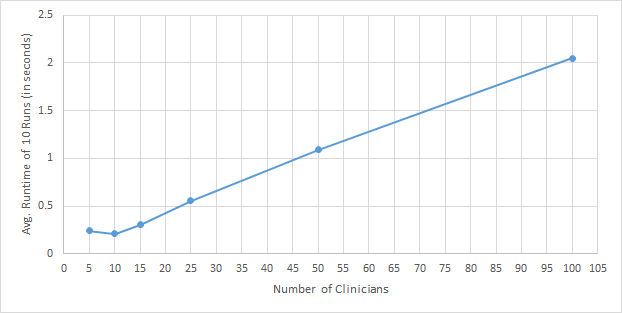
\includegraphics[scale=.7]{fig/avg_runtime_clinicians}
%	\caption{Plot of average runtime for LP with an increasing number of clinicians}
%	\label{fig:avg-runtime-clinicians}
%\end{figure}

%Next we evaluate the effect of increasing the number of departments. Figure \ref{fig:avg-runtime-divisions} shows the average runtime for a department with 10 clinicians, and a range of divisions, $D = \{1, 2, 3\}$. We can see that increasing the number of divisions even by 2 greatly affects the runtime. The LP solver had significant trouble when we increased the number of divisions further, making it impractical to quickly generate schedules for departments with many divisions. \\

%\begin{figure}[h]
%	\centering
%	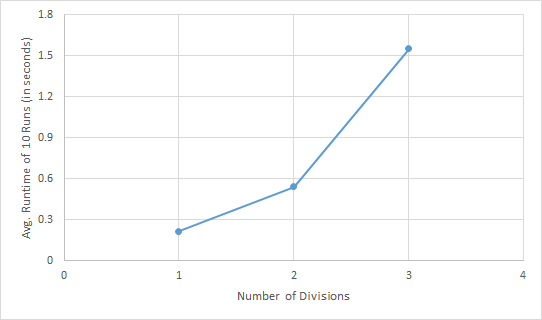
\includegraphics[scale=.7]{fig/avg_runtime_divisions}
%	\caption{Plot of average runtime for LP with an increasing number of divisions}
%	\label{fig:avg-runtime-divisions}
%\end{figure}

We plot the effect of an increasing number of requests per clinician on the average runtime of the LP solver in figure \ref{fig:avg-runtime-requests}. We run the program on a single-division department with 10 clinicians, and $R = \abs{\mathcal{WR}} + \abs{\mathcal{BR}} = \{1, 2, 3, 5, 10\}$ non-overlapping requests per clinician. The increase in the number of requests did not affect the runtime of the LP solver, indicating that it can accommodate a lot of flexibility in clinician requests. \\

\begin{figure}[h]
	\centering
	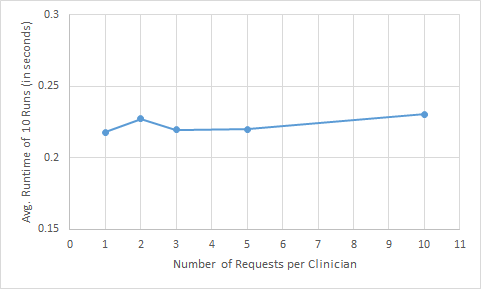
\includegraphics[scale=.7]{fig/avg_runtime_requests}
	\caption{Average runtime for LP with an increasing number of requests per clinician}
	\label{fig:avg-runtime-requests}
\end{figure}

We evaluate the effect of a longer time-horizon on the runtime of the algorithm. Figure \ref{fig:avg-runtime-blocks} presents the average runtime over 10 runs for an increasing number of 2-week blocks $B = \{26, 52, 78, 104\}$ to simulate a department that generates schedules for a few years in advance. We can see that there is an increasing trend in the runtime, however the solver is still able to find an optimal schedule for a 4-year time horizon in a very reasonable amount of time. \\

\begin{figure}[h]
	\centering
	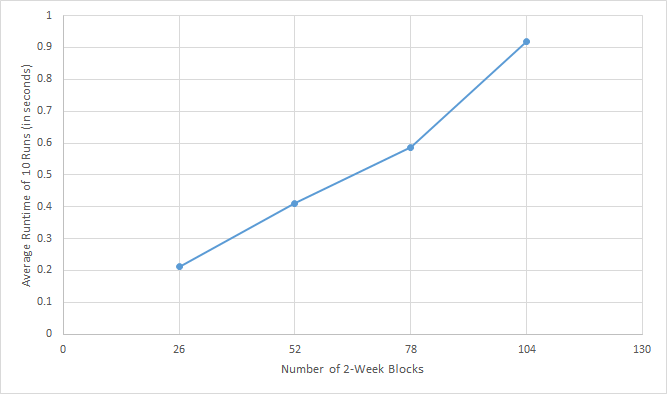
\includegraphics[scale=.7]{fig/avg_runtime_blocks}
	\caption{Average runtime for LP with an increasing number of 2-week blocks}
	\label{fig:avg-runtime-blocks}
\end{figure}

Lastly, we analyze the effect of increasing the number of divisions on the runtime of the program. Table \ref{tbl:runtime-divisions-comparison} presents the runtime for $D = \{1, 2, 3\}$ divisions and $C = \{10, 20, 30, 50\}$ clinicians in total across all divisions. For 2 divisions, a roster of more than 20 clinicians becomes impractical, if all constraints must be satisfied, but the runtime can be improved if we allow consecutive blocks to be assigned. For 3 divisions, the problem becomes impractical faster, with any more than 10 clinicians leading to unreasonable runtime for finding an optimal solution, and the problem cannot be improved by relaxing the consecutive blocks constraint.

\begin{table}
	\centering
	\begin{tabular}{|c|c|c|c|c|}
		\hline
		&       \multicolumn{4}{c|}{Number of Divisions}        \\ \hline
		Number of Clinicians &  1   &   2    & 2 (Consecutive Blocks Allowed) &  3   \\ \hline
		10          & 0.22 &  0.51  &              0.26              & 1.49 \\ \hline
		20          & 0.42 & 139.42 &              0.50              &     \\ \hline
		30          & 0.63 &   -    &              0.90              &     \\ \hline
		50          & 1.06 &   -    &              1.30              &     \\ \hline
	\end{tabular}
	\caption{Comparison of program runtime (in seconds) for different number of divisions and total clinicians. ``-'' indicates that a solution was not found after 24 hours.}
	\label{tbl:runtime-divisions-comparison}%
\end{table}


